\documentclass{standalone}
\usepackage{tikz}

\begin{document}
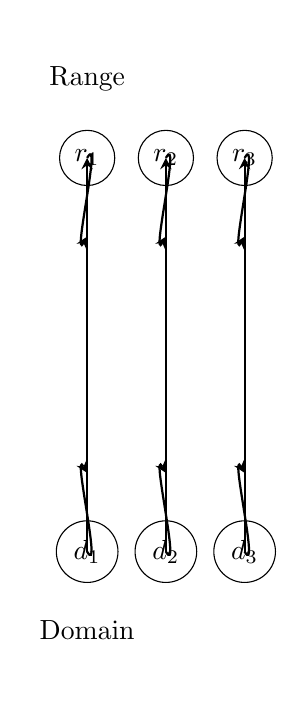
\begin{tikzpicture}[every node/.style={circle,draw}, 
                    arrow style/.style={->,thick,>=stealth}]
    % Define coordinates for the nodes
    \coordinate (D1) at (-2,-3);
    \coordinate (D2) at (-1,-3);
    \coordinate (D3) at (0,-3);
    
    \coordinate (R1) at (-2,2);
    \coordinate (R2) at (-1,2);
    \coordinate (R3) at (0,2);
    
    % Draw the domain set
    \node[draw=none] at (-2,-4) {Domain};
    \foreach \i in {1,...,3} {
        \node at (D\i) {$d_\i$};
        \draw[arrow style] (D\i) to[out=-60,in=120] ++(0,1);
    }
    
    % Draw the range set
    \node[draw=none] at (-2,3) {Range};
    \foreach \i in {1,...,3} {
        \node at (R\i) {$r_\i$};
        \draw[arrow style] (R\i) to[out=60,in=-120] ++(0,-1);
    }
    
    % Connect elements from domain to range
    \draw[arrow style] (D1) -- (R1);
    \draw[arrow style] (D2) -- (R2);
    \draw[arrow style] (D3) -- (R3);
\end{tikzpicture}
\end{document}